% CAP description for Button/Check Box/Radio Button
\begin{itemize}
\item This component includes standard buttons, check boxes and radio buttons.
\item A \bxname{Button} is a ''push'' button, 
usually manipulated with a click of the mouse over the button area:

\begin{figure}
\begin{center}
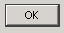
\includegraphics{PS/Button}
\caption{Button}
\label{button}
\end{center}
\end{figure}

\item A \bxname{Check Box} is commonly used to select or unselect an option (toggle):

\begin{figure}
\begin{center}
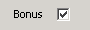
\includegraphics{PS/Checkbox}
\caption{Checkbox}
\label{checkbox}
\end{center}
\end{figure}

\item A \bxname{Radio Button} is used to choose one of a list of options:

\begin{figure}
\begin{center}
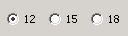
\includegraphics{PS/Radiobutton}
\caption{Radio Button}
\label{radiobutton}
\end{center}
\end{figure}

\end{itemize}
\clearpage
\textbf{Mapping buttons}

In the \gdomm{}, a button to be mapped looks like this:

\begin{figure}
\begin{center}
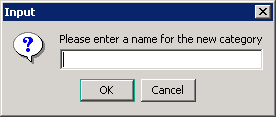
\includegraphics{PS/Mapbutton}
\caption{Button}
\label{mapbutton}
\end{center}
\end{figure}
